\documentclass[12pt, a4paper]{article}

\usepackage{statprojekt}
\newcommand{\naslov}{Projektna naloga iz Statistike}

\addbibresource{stat.bib}

\begin{document}

\author{Jan Pantner \\
\small Profesor: doc.~dr.~Martin~Raič}
\date{September 2024}
\maketitle
\thispagestyle{empty}

\newpage

\tableofcontents
\newpage

\section{Kibergrad}

Preučujemo dohodke družin v mestu Kibergrad. Imamo informacije o $43.886$ družinah, 
ki živijo v eni od štirih četrti: v severni četrti stanuje $10.149$ družin, v
vzhodni $10.390$, v južni $13.457$ in v zahodni $9.890$. Pomagamo si 
s programom \texttt{kibergrad.py}.

Iz vsake četrti vzemimo enostavni slučajni vzorec velikosti $100$. 
Dohodke primerjamo s pomočjo škatel z brki, o katerih je več 
napisano v \cite[Poglavje~10.6]{rice2007mathematical}.
Vzporedne škatle z brki so prikazane na sliki \ref{img:cetrti}.
\begin{figure}[H]
    \centering
    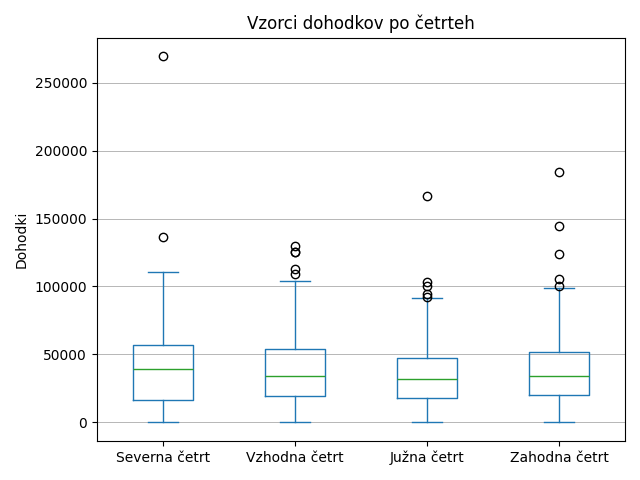
\includegraphics[width=12cm]{Slike/vse_cetrti.png}
    \caption{Škatle z brki za dohodke posamezne četrti.}
    \label{img:cetrti}
\end{figure}
Najprej opazimo, da je v severni četrti osamelec, ki močna izstopa. Prav tako so maksimum, tretji 
kvartil in mediana v severni četrti največji, vendar razlika ni dovolj velika, 
da bi lahko pri tako majhnem vzorcu sklepali, da so dohodki severne četrti 
najvišji. Zdi pa se, da so dohodki severne četrti malenkost višji kot dohodki 
južne četrti, pri kateri so vse prej omenjene vrednosti najmanjše. 

Zdi se, da v splošnem četrt ne vpliva močno na velikost dohodka.

Sedaj vzemimo še štiri enostavne slučajne vzorce velikosti $100$ 
iz severne četrti in poglejmo vzporedne škatle z brki za vzorce
iz severne četrti. Prikazane so na sliki \ref{img:sever}.
\begin{figure}[H]
    \centering
    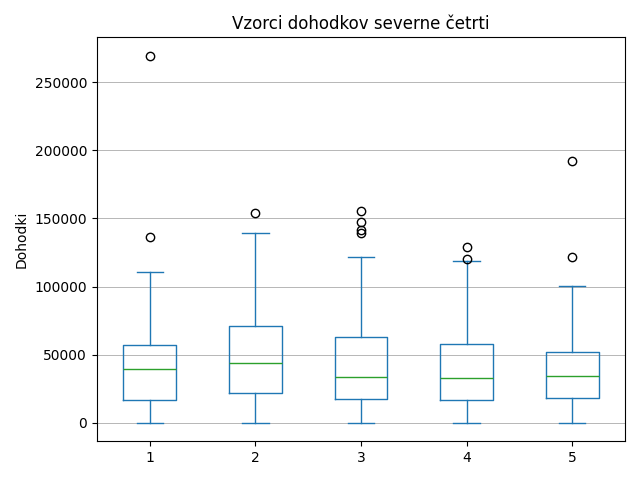
\includegraphics[width=12cm]{Slike/sever.png}
    \caption{Škatle z brki dohodkov severne četrti.}
    \label{img:sever}
\end{figure}
Vse mediane so večje od $33.000$, njihovo povprečje je približno 
$36.500$. Zdi se, da lahko s precejšnjo sigurnostjo sklepamo, da je večina 
dohodkov višjih od $33.000$.

V novih vzorcih ne opazimo tako ekstremnih osamelcev kot pri prvem vzorcu. Večina 
osamelcev ni zelo oddaljenih od maksimuma.

Za konec si poglejmo še varianco dohodka pojasnjeno s četrtmi in preostalo
(rezidualno) varianco. Naj bo $N$ velikost populacije, $N_i$ velikost 
populacije $i$-te četrti in $w_i$ velikostni delež $i$-te četrti. Naj bo
$\mu$ povprečni dogodek in $\sigma^2$ varianca dohodka Kibergrada,
$\mu_i$ in $\sigma_i^2$ pa zaporedoma povprečni dohodek in varianca 
dohodka $i$-te četrti. 
Pojma pojasnjene in nepojasnjene variance sta razložena v 
\cite{raic}. Zaporedoma sta določena s formulama
\[
    \sigma^2_B := \sum_{i=1}^{4} w_i(\mu_i - \mu)
    \quad \text{in} \quad
    \sigma^2_W := \sum_{i=1}^{4} w_i\sigma_i^2.
\]
Izračunamo, da je 
\[
    \sigma^2_B = 9.252.923
    \quad \text{in} \quad
    \sigma^2_W = 1.017.226.451.
\]
S četrti pojasnjeni 
standardni odklon je torej $3.042$. Povprečni dohodki četrti, 
so enaki $45.759$, $41.235$, $37.473$ in $42.158$, torej je 
standardni odklon v primerjavi z njimi majhen. To se ujema z 
opažanjem, da četrt ne vpliva močno na velikost dohodka.
\newpage

\section{Lomljivost najlonskih palic}
Na vzorcu $280$ najlonskih palic preizkušamo njihovo lomljivost. Rezultati 
preizkusa so prikazani v tabeli \ref{table:lomljivost}. Pri analizi 
si pomagamo s programom $\texttt{najlonske\_palice.py}$.
\begin{table}[H]
    \centering
    \begin{tabular}{|l||l|l|l|l|l|l|}
        \hline
        št.~lomov & 0   & 1  & 2  & 3  & 4 & 5 \\ \hline
        št.~palic & 157 & 69 & 35 & 17 & 1 & 1 \\ \hline
    \end{tabular}
    \caption{Rezultati preizkusa lomljivosti.}
    \label{table:lomljivost}
\end{table}
Privzemimo, da je število mest, na katerih se je palica 
zlomila porazdeljeno binomsko $\Bin(5, p)$ za določen neznan $p$.
Privzemimo tudi, da so palice med seboj neodvisne.

%-----------------------  Naloga (a) -----------------------%

Pri teh predpostavkah je logaritem verjetja podan z
\[
    l(p, x) = \log\prod_{i=1}^{280} \binom{5}{x_i}p^{x_i}(1-p)^{5-x_i}.
\]
Izračunamo, da je maksimum 
dosežen pri $\hat p = 0{,}14214$. Ta vrednost
nam predstavlja oceno $p$ po metodi največjega verjetja.

%-----------------------  Naloga (b) -----------------------%

Sedaj združimo zadnje tri vrednosti in preizkusimo ničelno domnevo, da 
je število mest, na katerih se je palica zlomila porazdeljeno 
binomsko $\Bin(5, p)$ proti alternativni domeni, da ima število 
lomov katero drugo porazdelitev.
To storimo s Pearsonovim preizkusom hi kvadrat, ki je podrobneje
opisan v \cite[Poglavje~9.5]{rice2007mathematical}.

Pearsonova testna statistika je
\[
    X^2 = \sum_{i=0}^{2}\frac{(x_i - nf_i(\hat p))^2}{nf_i(\hat p)},
\]
kjer je $x_0 = 157$, $x_1 = 69$, $x_2 = 35$, $x_3 = 19$ in
\[
    f_i(\hat p) = \begin{cases}
        \binom{5}{x_i}\hat p^{x_j}(1-\hat p)^{5-x_i}, &i \in \set{0,1,2} \\
        \sum_{j=3}^{5} \binom{5}{x_j}\hat p^{x_j}(1-\hat p)^{5-x_j}, &i = 3 
    \end{cases}.
\]
Izračunamo, da je $X^2 > 44$. Iz tabela kvantilov porazdelitve 
hi kvadrat sledi, da ničelno domnevo zavrnemo tako 
pri stopnji tveganja $\alpha = 0{,}01$ kot tudi pri $\alpha = 0{,}05$. 

%-----------------------  Naloga (c) -----------------------%

Recimo sedaj, da imamo za $i = 1, \dots, 280$ neodvisna opažanja
$X_i \sim \Bin(m_i, p_i)$, kjer so parametri $m_i$ znani, 
$p_i$ pa neznani. S pomočjo razmerja verjetih preizkusimo 
ničelno domnevo, da so vsi parametri $p_i$ enaki, proti 
alternativni domnevi, da temu ni tako.

Verjetja sta enaka
\begin{align*}
    L_1 = \prod_{i=1}^{280} \binom{m_i}{x_i}p_i^{x_i}(1-p_i)^{m_i-x_i} \\
    L_0 = \prod_{i=1}^{280} \binom{m_i}{x_i}p_0^{x_i}(1-p_0)^{m_i-x_i}   
\end{align*}
Torej je razmerje verjetij enako
\[
    \Lambda =
    \frac{\prod_{i=1}^{280} \hat p_i^{x_i}(1-\hat p_i)^{m_i-x_i}}
    {\prod_{i=1}^{280} \hat p_0^{x_i}(1-\hat p_0)^{m_i-x_i}}
\]
Če logaritem verjetja $L_1$ odvajamo po $p_i$ 
dobimo
\[
    \frac{x_i}{p_i} - \frac{x_i-m_i}{1-p_i}.
\]


\boxed{\texttt{TO DO}}


\newpage

\section{Spreminjanje temperature v Ljubljani}

V tem razdelku preučujemo spreminanje temperature v Ljubljani s 
pomočjo podatkov izmerjenih mesečno v letih od $1994$ do $2023$.
Pomagamo si s programom \texttt{temperature.py}.

Najprej predpostavimo linearni trend in sinusno nihanje s periodo eno leto. 
To nam da model
\[
    y_{l,m} = Ax_l + B\sin(x_m\pi/6 + \delta) + C
\]
oziroma
\[
    y_{l,m} = Ax_l + B\sin(x_m\pi/6) + C\cos(x_m\pi/6) + D,
\]
kjer je $x_l$ leto meritve, $x_m$ mesec meritve, $y_{l,m}$ pa 
izmerjena temperatura v tem mesecu tega leta. Več o sinusnem 
modelu v \cite{wiki:Sinusoidal_model}. Alternativno je model 
dolečen z
\[
    Y = X_A\beta_A,
\]
kjer je $\beta_A^\top = \begin{bmatrix}
    D & C & B & A
\end{bmatrix}$ in
\[
    X_A = \begin{bmatrix}
        1 & 1 & 0 & 1 \\
        1 & 1 & \sin\left(\pi/6\right) & \cos\left(\pi/6\right) \\
        \vdots & \vdots & \vdots & \vdots \\
        1 & 1 &  \sin\left(11\pi/6\right) & \cos\left(11\pi/6\right) \\
        1 & 2 & 0 & 1 \\
        \vdots & \vdots & \vdots & \vdots \\
        1 & 2 &  \sin\left(11\pi/6\right) & \cos\left(11\pi/6\right) \\
        1 & 3 &  0 & 1 \\
        \vdots & \vdots & \vdots & \vdots \\
        1 & 30 & \sin\left(11\pi/6\right) & \cos\left(11\pi/6\right)\\
        \end{bmatrix}.
\]
Torej, $X_A$ je matrika velikosti $360 \times 4$. Predpostavimo, da je 
naš model Gaussov. Tedaj je ocena za $\beta_A$ po metodi največjega 
verjetja enaka
\[
    \hat \beta_A = (X_A^\top X)^{-1} X^\top Y.
\]
Izračunamo
\[
    \beta_A^\top = \begin{bmatrix}
        10.747 & 0.056 & 0.039 & -10.379
    \end{bmatrix}.
\]
Prva komponenta nam pove, da imamo pozitiven trend, kar se zdi 
smiselno. Kako dober je model lahko ocenimo s pomočjo slike 
\ref{png:prvi}.
\begin{figure}[H]
    \centering
    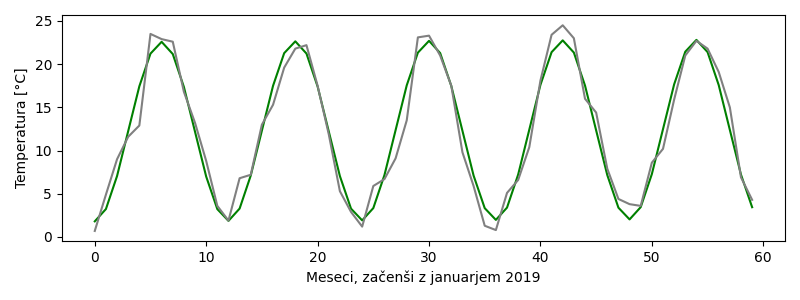
\includegraphics[width=14cm]{Slike/prvi_model.png}
    \caption{Siva krivulja označuje izmerjene podatke, zelena pa oceno 
    prvega modela.}
    \label{png:prvi}
\end{figure}
Alternativno predpostavimo linearni trend temperature za 
vsak mesec v letu posebej. V tem primeru dobimo matriko
\[
    X_B = \begin{bmatrix}
        1 & 1 & 0 & 0 & \cdots & 0 & 0 \\
        1 & 0 & 1 & 0 & \cdots & 0 & 0 \\
        \vdots & & & & \ddots & & & \\
        1 & 0 & 0 & 0 & \cdots & 0 & 1 \\
        1 & 2 & 0 & 0 & \cdots & 0 & 0 \\
        \vdots & & & & \ddots & & & \\
        1 & 0 & 0 & 0 & \cdots & 0 & 2 \\
        1 & 3 & 0 & 0 & \cdots & 0 & 0 \\
        \vdots & & & & \ddots & & & \\
        1 & 0 & 0 & 0 & \cdots & 0 & 30 
    \end{bmatrix},
\]
ki je velikosti $360 \times 13$. Izračunamo
\setcounter{MaxMatrixCols}{20}
\footnotesize
\[
    \beta_A^\top = \begin{bmatrix}
        10.75 & -0.46 & -0.37 & -0.17 & 0.05 & 0.26 & 
        0.50 & 0.58 & 0.54 & 0.29 & 0.06 & -0.19 & -0.42
    \end{bmatrix}.
\]
\normalsize
Za model očitno ni preveč dober. To lahko vidimo tudi na sliki 
\ref{png:drugi}.
\begin{figure}[H]
    \centering
    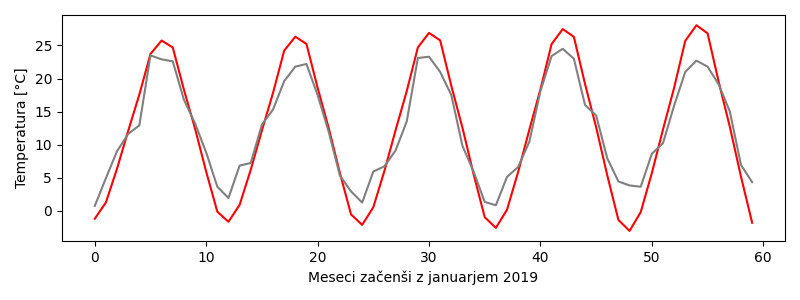
\includegraphics[width=14cm]{Slike/drugi_model.png}
    \caption{Siva krivulja označuje izmerjene podatke, rdeča pa oceno 
    drugega modela.}
    \label{png:drugi}
\end{figure}
Takšna razlika se verjetno pojavi zaradi avtorjeve napačne interpretacije navodil 
projektne naloge. Verjetno je mišljeno, da je drugi model določen z matriko
\[
    X_C = \begin{bmatrix}
        1 & 1 & 0 & 0 & \cdots & 0 & 0 \\
        1 & 0 & 1 & 0 & \cdots & 0 & 0 \\
        \vdots & & & & \ddots & & & \\
        1 & 0 & 0 & 0 & \cdots & 0 & 1 \\
        2 & 1 & 0 & 0 & \cdots & 0 & 0 \\
        \vdots & & & & \ddots & & & \\
        2 & 0 & 0 & 0 & \cdots & 0 & 1 \\
        3 & 1 & 0 & 0 & \cdots & 0 & 0 \\
        \vdots & & & & \ddots & & & \\
        30 & 1 & 0 & 0 & \cdots & 0 & 1 
    \end{bmatrix}.
\]
To je ponovno matrika velikosti $360 \times 13$. V tem primeru je
\footnotesize
\[
    \beta_A^\top = \begin{bmatrix}
        0.06 & 0.26 & 2.14 & 6.30 & 10.68 & 15.29 & 
        19.56 & 21.21 & 20.48 & 15.44 & 10.88 & 5.82 & 0.92
    \end{bmatrix}
\]
\normalsize
Prva komponenta nam pove, da imamo pozitiven linearen trend, 
iz ostalih komponent pa je lepo razvidno kako se temperature
spreminjajo skozi mesece. Res na primer vidimo, da model 
predvide najnižje temperature pozimi in najvišje poleti.
Model je prikazan na sliki \ref{png:tretji}.
\begin{figure}[H]
    \centering
    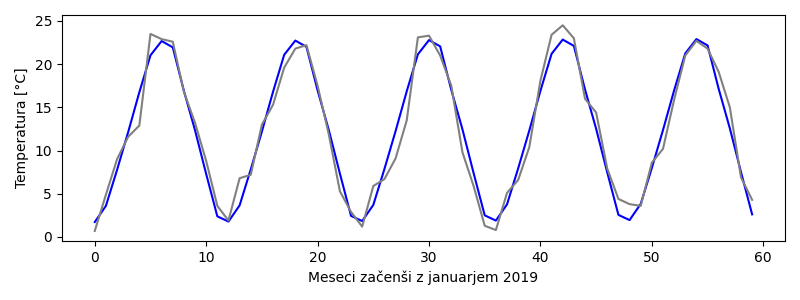
\includegraphics[width=14cm]{Slike/tretji_model.png}
    \caption{Siva krivulja označuje izmerjene podatke, modra pa oceno 
    tretjega modela.}
    \label{png:tretji}
\end{figure}
Tretji model je širši od prvega. Preizkusimo model $A$ znotraj 
modela $C$, torej preizkusimo ničelne domnevo, da velja model $A$, 
proti alternativni, da velja model $B$ z odvzetim podmodelom $A$.
To lahko storimo na podlagi statistike
\[
    F := \frac{(\RSS_A - \RSS_C)(n-p)}{\RSS_C (p-q)},
\]
kjer sta $p$ in $q$ prostorski stopnji modelov $C$ in $A$. 
Ničelno domnevo zavrnemo, če je 
\[
    F \ge F^{-1}_{\fish(p-q,n-p)}(1-\alpha),
\]
kjer je $\alpha$ stopnja tveganja. 
Izpeljava je na voljo v \cite{raic2}. 

V našem primeru je $p = 13$ in $q = 4$. Izračunamo 
\[
    F = 1{,}595, \quad
    F^{-1}_{\fish(9,347)}(1-0{,}05) = 1{,}907 \quad \text{in} \quad
    F^{-1}_{\fish(9,347)}(1-0{,}01) = 2{,}459.
\]
Ničelne domneve torej ne moremo zavrniti.
% F = (RSS_A - RSS_C) * (n-p) / (p-q) / RSS_C

\subsection*{Določanje optimalnega modela s Akaikejevo informacijo}

Pri izbiri boljšega modela si lahko pomagamo z Akaikejevo informacija, 
ki je v primeru linearne regresije in Gaussovega modela enaka
\[
    \AIC := 2p + n \ln \RSS,
\]
kjer je $p$ število parametrov, $n$ število opažanj in $\RSS = \norm{Y - X\hat \beta}$.

Akaikejeva informacija prvega modela je enaka $1261$,
tretjega pa $1265$. Torej ima model $A$ malenkost
manjšo Akaikejevo informacijo in je primernejši.

Akaikejeva infromacija drugega modela je enaka $1577$. 
To se sklada z opažanjem iz slike, da je drugi model bistveno
slabši od prvega (in tretjega).

Kot zanimivost slika \ref{png:cetrti} prikazuje kaj se zgodi, 
če matriki $X_C$ na začetek dodamo še stolpec enic.
Nepresenetljivo, glede na sliko, je Akaikejeva infromacija tega modela veliko 
večja od prejšnih -- enaka je $2330$.
\begin{figure}[H]
    \centering
    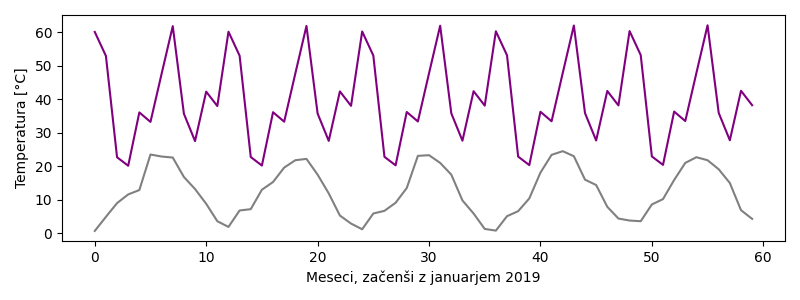
\includegraphics[width=14cm]{Slike/cetrti_model.png}
    \caption{Siva krivulja označuje izmerjene podatke, vijolična pa oceno 
    četrtega modela.}
    \label{png:cetrti}
\end{figure}

\newpage

\nocite{*}
\printbibliography
\addcontentsline{toc}{section}{Literatura}

Kvantili Fisherjeve porazdelitve so bili izračunani s kalkulatorjem Stat Trek
dostopnim na \url{https://stattrek.com/online-calculator/f-distribution}.


\end{document}